\documentclass[12pt]{article}

\usepackage[onlytext]{MinionPro}
\usepackage{microtype}                                                          % Better looking documents "typographical perfection"

\usepackage[left=3cm, right=3cm]{geometry}		                                % Margins left and right
\usepackage{hyperref}                                                           % Clickable table of contents in PDFs
\usepackage{datetime}                                                           % Currenttime
\usepackage[titletoc,title]{appendix}                                           % Appendices in table of contents

\usepackage{graphicx}                                                           % Include figures
\usepackage{float}                                                              % Better float options: H(ere)
\usepackage[most]{tcolorbox}                                                    % Breakable box for digressions

\usepackage{physics}                                                            % Physics typesetting: bra-ket
\usepackage{mathtools}                                                          % for the custom command \set and
                                                                                % package amsmath: \tag
\usepackage{xparse}                                                             % for the custom command \set
\usepackage{mathrsfs}                                                           % \mathsrc
\usepackage{amssymb}                                                            % \mathbb
\usepackage{amsthm}                                                             % \qedhere
\usepackage{interval}

\numberwithin{equation}{section}                                                % Equations are numbered per section
\numberwithin{figure}{section}                                                  % Figures are numbered per subsection

\setlength{\parindent}{0in}                                                     % No indentation for every paragraph
  % Packages for this project
% % % Special notations for sets of numbers
\newcommand{\N}{\mathbb{N}}                                                     % Natural numbers
\newcommand{\R}{\mathbb{R}}                                                     % Real numbers
\newcommand{\C}{\mathbb{C}}                                                     % Complex numbers
\newcommand{\F}{\mathbb{F}}                                                     % General field, R or C

% % % Special notations for groups
\DeclareMathOperator{\GLg}{GL}                                                  % General linear group
\DeclareMathOperator{\SLg}{SL}                                                  % Special linear group
\DeclareMathOperator{\Og}{O}                                                    % Orthogonal group
\DeclareMathOperator{\SOg}{SO}                                                  % Special orthogonal group
\DeclareMathOperator{\Ug}{U}                                                    % Unitary group
\DeclareMathOperator{\SUg}{SU}                                                  % Special unitary group
\DeclareMathOperator{\Aut}{Aut}                                                 % The automorphism group

% % % Other math operators
\DeclareMathOperator{\id}{id}                                                   % Identity function
\DeclareMathOperator{\diag}{diag}                                               % Diagonal matrix


% Create a custom command for set notation
%
\DeclarePairedDelimiterX{\set}[1]{\{}{\}}{\setargs{#1}}
\NewDocumentCommand{\setargs}{>{\SplitArgument{1}{;}}m}
{\setargsaux#1}
\NewDocumentCommand{\setargsaux}{mm}
{\IfNoValueTF{#2}{#1} {#1\,\delimsize|\,\mathopen{}#2}}%{#1\:;\:#2}
  % Custom commands for this project


\title{Mathematics}
\author{Laurent Lemmens \\ GQCG}
\date{\today \hspace{6pt} \currenttime}


\begin{document}

\maketitle

% % % ABSTRACT AND TABLE OF CONTENTS

% Abstract
\begin{abstract} \noindent  % enters inside the abstract are not rendered as line breaks in the .pdf-file
    These notes serve as a summary of mathematics I have thorougly studied.
\end{abstract}

% Line after abstract
\begin{center}
    \line(1,0){250}
\end{center}

% Table of contents
\tableofcontents
\newpage



% % % MAIN TEXT % % %

\newpage
\section{Functions - relations between sets}
    \subsection{Sets}
        Modern algebra starts from the notion of a set. A set $S$ is a collection of elements:
        \begin{equation}
            S = \set{s_1, s_2, \dots, s_n} \thinspace .
        \end{equation}
        Some examples of sets are the set of natural numbers $\N$, the set of real numbers $\R$, the set of complex numbers $\C$. We can also have smaller sets, for example
        \begin{equation}
            S = \set{0, 1} \thinspace ,
        \end{equation}
        being the set of the numbers $0$ and $1$. Sets don't necessarily have to contain only numbers. We can, for example, collect all invertible $n \times n$-matrices in a set:
        \begin{equation}
            \GLg(n, \mathbb{R}) = \set{A \in \mathbb{R}^{n \times n} ; \text{$A$ is invertible}} \thinspace ,
        \end{equation}
        in which the symbol $\GLg$ has to do with `general linear', but more on that when we encounter the general linear group. \\

        The previous examples are all concrete (i.e. not abstract) examples of sets. Now say we have a mathematical object, called $E$ (we haven't specified anything about it), we can say that
        \begin{equation}
            G = \set{E}
        \end{equation}
        is also a set, but in a more abstract sense than the previous examples. We can enlarge this set by adding the elements $C_2, \sigma_v$ and $\sigma_v'$, to end up with
        \begin{equation}
            G = \set{E, C_2, \sigma_v, \sigma_v'} \thinspace ,
        \end{equation}
        in which we still haven't specified anything about the nature of its elements, but in mathematics that is perfectly fine. \\

    \subsection{Functions - introduction}
        Naturally, if we have two different sets, we would like to be able to define relations between their elements. This is exactly what a function does. A function (or map, mapping, these are all synonyms) is a relation between two sets $X$ and $Y$:
        \begin{equation} \label{eq:def_function}
            f: X \rightarrow Y: x \mapsto y = f(x) ,
        \end{equation}
        subject to the important condition that every input $x \in X$ is related to exactly one output $y \in Y$. We would read the definition in equation (\ref{eq:def_function}) as follows: $f$ is a function from the set $X$ to the set $Y$, in which every $x \in X$ is related to a $y \in Y$, which we call $f(x)$. \\

        We give special names to the sets $X$ and $Y$, depending on which role they play in the function. The set $X$ is called the domain of the function: it is the set of all inputs for the function. The set $Y$ is then called the function's codomain: it is the set of values that \emph{could} occur as output values for the function. We can then define another set, $Z$, which is called the image of the function: it is the set of \emph{actual} values for the outputs. A visual clarification of the terms can be found in Figure \ref{fig:functions}. \\
        \begin{figure}[H] \centering
            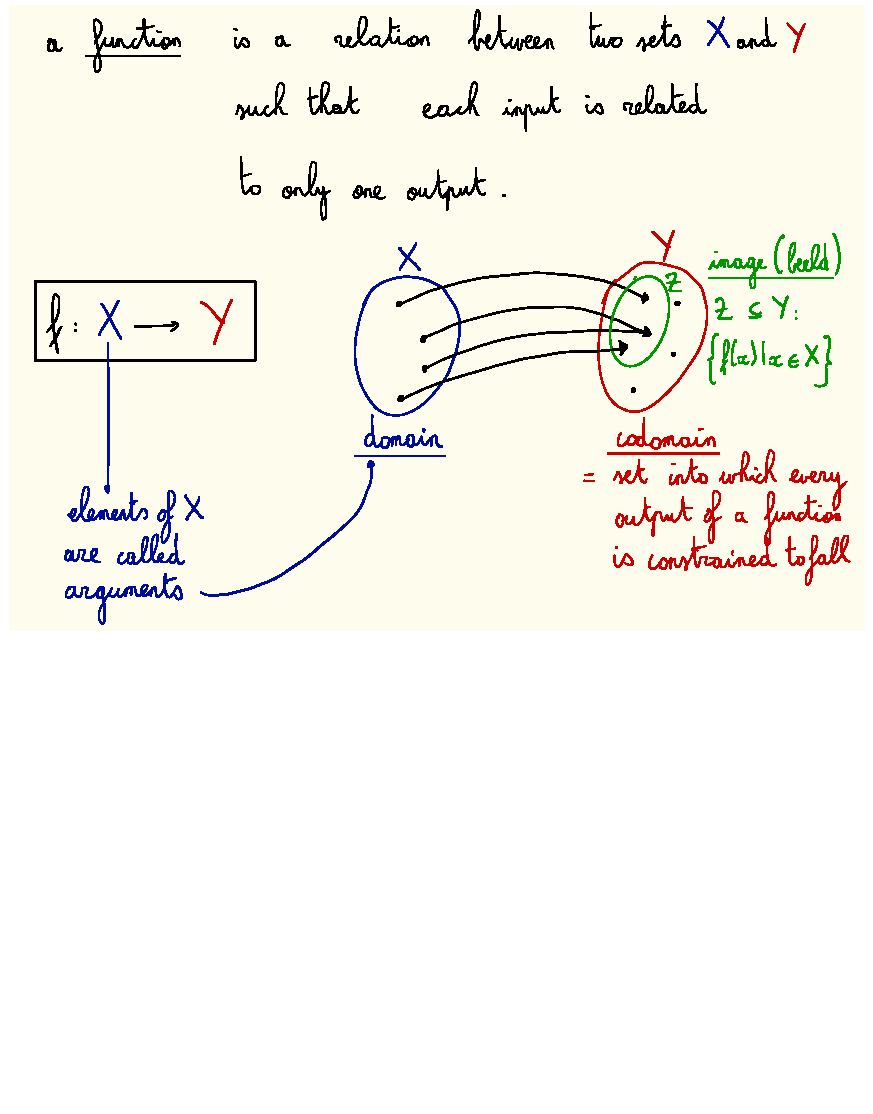
\includegraphics{images/functions}
            \caption{The definition of a function, and a visual clarification of the terms domain, codomain and image. The domain is the set of input values, the codomain is the set of possible output values, and the images is the set of actual output values.}
            \label{fig:functions}
        \end{figure}

        An example of a function could be:
        \begin{equation}
            f: \R \rightarrow \R: x \mapsto f(x) = x^2 + 2
        \end{equation}
        Its domain is $\R$, and its codomain is also $\R$. Here, we can also see the difference between the codomain and the image. The codomain of this function is defined to be $\R$, but its image $[2, +\infty[$. Another example is shown in Figure \ref{fig:function_color}.
        \begin{figure}[H] \centering
            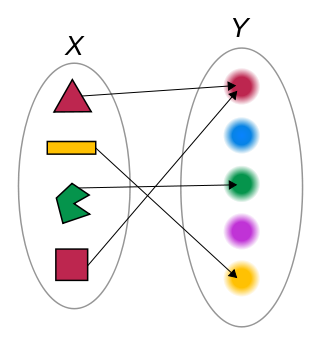
\includegraphics[scale=0.4]{images/function_color}
            \caption{An example of a function that maps an object to its color.}
            \label{fig:function_color}
        \end{figure}
        The reason why this is a function is because every input element of the set $X$, being shapes in a certain color, is related to its color, represented as elements of the set $Y$. In this case, $Y$, the codomain is the set of colors depicted as elements of $Y$, and the range is the set of colors red, green and yellow. \\

        We have seen some examples of functions already, but what are some examples relations that are not functions? There are actually two requirements to the definition of a function:
        \begin{enumerate}
            \item Every input (element of the domain) has to be related to an output (element of the codomain)
            \item No two outputs (elements of the codomain) may be related to the same input (element of the domain)
        \end{enumerate}
        With these two criteria in mind, it is possible to come up with many examples of relations between two sets that are not functions, for example those shown in Figure \ref{fig:non_functions}.
        \begin{figure}[H] \centering
            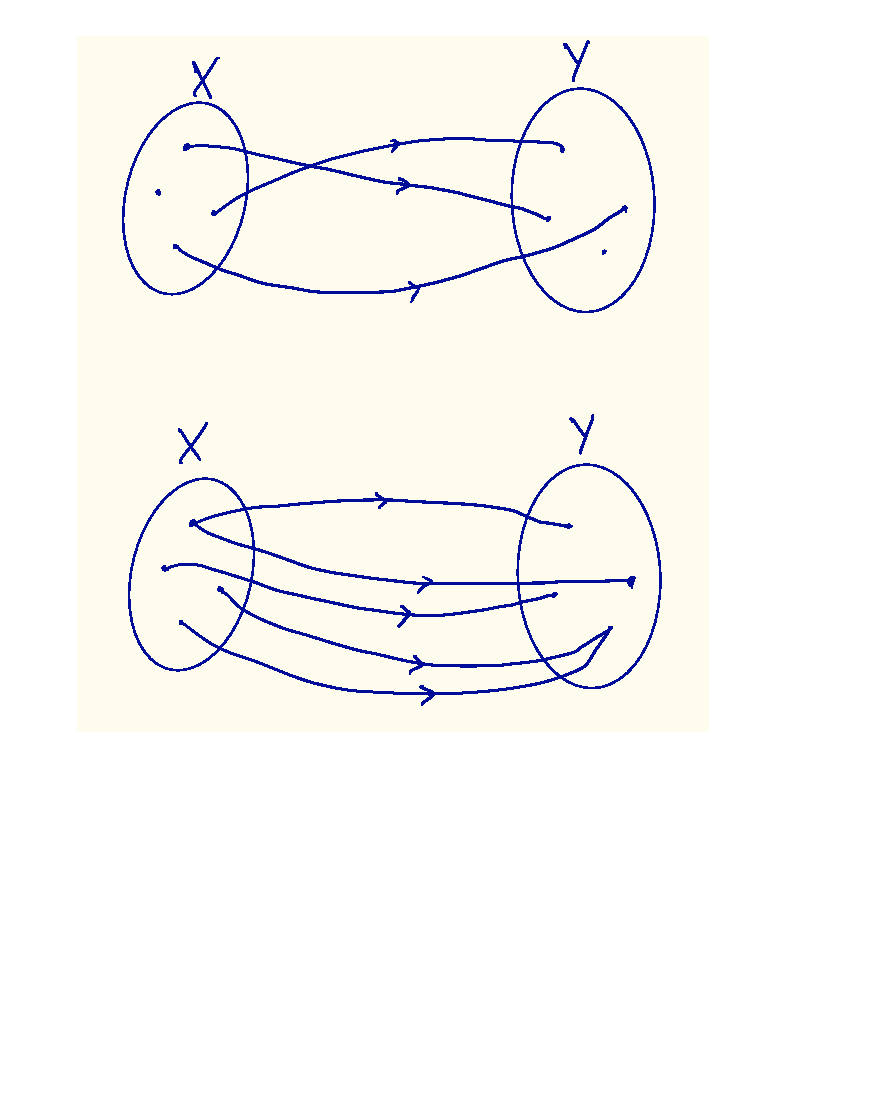
\includegraphics{images/non_functions}
            \caption{Two examples of non-functions. The first relation between $X$ and $Y$ is not a function, because not every element of $X$ is related to an element of $Y$. The second figure is not a function because there is an element of $X$ related to two elements of $Y$.}
            \label{fig:non_functions}
        \end{figure}

        The identity function on a set $S$ is the function:
        \begin{equation}
            \id_S: S \rightarrow S: \id_S(s) = s \thinspace .
        \end{equation}

        An operation can hardly be distinguished from the definition of a function that was already given. It is a function
        \begin{equation}
            \omega: Y_1 \times \cdots \times Y_N \rightarrow X \thinspace ,
        \end{equation}
        which takes as an input one element of every of its input sets $Y_i$ and relates that combination to the output set $X$. For me, this definition is exactly equal to the definition that was given previously. However, it seems that the term operation is often used to talk about associativity, commutativity, etc. \\

        We know many operations, for example number addition, which takes two numbers as input and relates that combination to a number. Number multiplication is another example of a binary operation: we take two numbers, whose product is a number. If we take, for example, set of $n \times n$ matrices, then matrix multiplication is an example of a binary operation. Furthermore, we don't have to take inputs from the same sets! We can define scalar multiplication as an operation that relates a number and a vector to a vector. \\

    \subsection{Classification of functions}
        By now, we have seen some examples of functions. In order to classify functions, we will introduce the terms surjection, injection, and bijection. For a visual overview of the terms, see Figure \ref{fig:sur_in_bi}. \\

        A function is called surjective (or: onto), if every element of its codomain is mapped to. \emph{Sur} means `above', which relates to the fact that the function's codomain is completely covered. Its definition can be written as follows: a function $f$ is said to be surjective if
        \begin{equation}
            f: X \rightarrow Y: \forall y \in Y: \exists x \in X: f(x) = y \thinspace .
        \end{equation}

        A function is called injective (or: one-to-one) if no element of its codomain is mapped to twice. Mathematically, we would write: $f$ is an injective function if
        \begin{equation}
            f: X \rightarrow Y: \forall a, b \in X: f(a) = f(b) \Rightarrow a = b \thinspace .
        \end{equation}

        A function is called bijective (or: one-to-one and onto, a one-to-one correspondence), if it is both injective and surjective: every element of the codomain is mapped to by exactly one element of the domain. \\

        \begin{figure}[H] \centering
            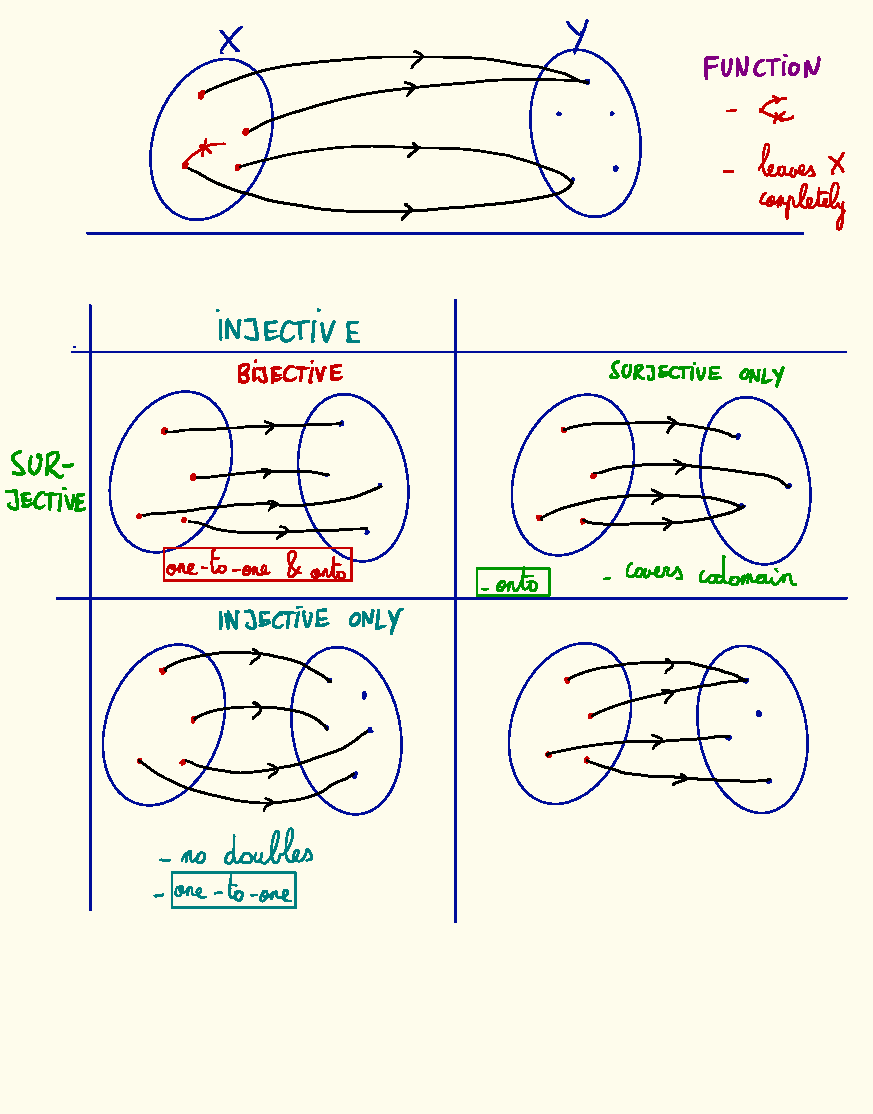
\includegraphics{images/sur_in_bi}
            \caption{A visual scheme of the terms surjective, injective and bijective.}
            \label{fig:sur_in_bi}
        \end{figure}

        Given Figure \ref{fig:sur_in_bi}, we can already see examples of surjective and injective functions. In Figure \ref{fig:function_color}, we can see an example of a function that is not surjective (not every color is mapped to), nor injective (the color red is mapped to twice). \\


\newpage
\section{Algebraic structures}
    Algebraic structures are a combination of a set, together with one or more operations, satisfying a list of axioms.

    \subsection{The mathematical definition of a group} \label{sec:group_def}
        A group has a mathematical definition. It is a set $G$\footnote{We often use the same symbol to denote the set of group elements and the actual group. I don't think there is anything wrong with this, as the distinction is most often clear from the context.} with elements $G=\set{g_1, g_2, \dots, g_n}$, together with an operation $\cdot$ (which is often called the group multiplication), meeting the following axioms:
        \begin{enumerate}
            \item closedness
            \begin{equation}
                \forall g_1, g_2 \in G: g_1 \cdot g_2 \in G
            \end{equation}

            \item associativity
            \begin{equation}
                \forall g_1, g_2, g_3 \in G: g_1 \cdot (g_2 \cdot g_3) = (g_1 \cdot g_2) \cdot g_3
            \end{equation}

            \item identity element
            \begin{equation} \label{eq:group_id}
                \exists! \thinspace e \in G: \forall g \in G: e \cdot g = g \cdot e = g
            \end{equation}

            \item inverses
            \begin{equation}
                \forall g \in G: \exists! \thinspace g^{-1} \in G: g \cdot g^{-1} = g^{-1} \cdot g = e
            \end{equation}
        \end{enumerate}
        If the axiom
        \begin{enumerate}
            \setcounter{enumi}{4}
            \item commutativity
            \begin{equation}
                \forall g_1, g_2 \in G: g_1 \cdot g_2 = g_2 \cdot g_1
            \end{equation}
        \end{enumerate}
        is also met, the group is called Abelian. \\

    \subsection{Examples of groups}
        Since the definition of a group is so abstract, let us try to examine some examples of groups. \\

        As a first, let us consider a group that is familiar to all of us. Let us take the set $\mathbb{R}_0$: the rational numbers excluding $0$, together with the operation of multiplication. We can check that every group axiom holds (the identity element is $1$, and we know the inverse of every real number), even the commutative one. We can therefore say that $\mathbb{R}_0$ with multiplication is an Abelian group. \\

        In section \ref{sec:group_def}, we gave a general name to the group operation: group multiplication. This doesn't mean that the group operation can't be addition, for example, as `group multiplication' is just a name. A perfectly valid example of an Abelian group is the set of integers $\mathbb{Z}$, together with addition. Again, we can check that all group axioms hold (the identity element is $0$, and we all know the inverse of integers with respect to addition). \\

        As a slightly more complicated example of a group, we will consider the general linear group over $\mathbb{R}$ of degree $n$, denoted by $\GLg(n, \mathbb{R})$. This is the set of all invertible $n \times n$-matrices with real entries, with the operation of matrix multiplication. The identity element is $I_n$: the $n \times n$-identity matrix (a diagonal matrix with $1$ on the diagonal), and since we have specified the set as being the set of invertible matrices, every matrix has an inverse. We should emphasize that $\GLg(n, \mathbb{R})$ is not Abelian, as, in general, matrix multiplication is not commutative. A special case of this group is formed by requiring that the determinant of the invertible $n \times n$-matrices is equal to $1$. We call this set of matrices, together with matrix multiplication, the special linear group $\SLg(n)$. \\

        Many sets of matrices, together with the operation of multiplication form a group. We have for example $\Og(n)$, being the set of $n \times n$ orthogonal ($Q^\text{T} Q = Q Q^\text{T} = I_n$) matrices under matrix multiplication. A special group that is related to $\Og(n)$ is $\SOg(n)$, being the set of orthogonal matrices with determinant equal to $1$, under matrix multiplication. Furthermore, we also have the group $\Ug(n)$, being the set of $n \times n$ unitary matrices ($U U^\dagger = U^\dagger U = I_n$), under the group operation of matrix multiplication. Again, a special variant is $\SUg(n)$, being the set of $n \times n$ unitary matrices with determinant equal to $1$, under matrix multiplication. \\

        As a first more abstract example, let us take a look at the trivial group. It consists of the set $G = \set{e}$ under group multiplication. We have to specify that $e$ is the element for which equation (\ref{eq:group_id}) holds: $e$ is the identity element, and consequently its own inverse. With this in mind, we can check that the trivial group is Abelian. \\

        As another abstract example, let's take the set of elements
        \begin{equation}
            G = \set{E, C_2, \sigma_v, \sigma_v'} \thinspace ,
        \end{equation}
        with the multiplication table given in Table \ref{table:multiplication_table_C2v}.
        \begin{table}[H] \centering
            \begin{tabular}{r|rrrr}
                            & $E$           & $C_2$         & $\sigma_v$    & $\sigma_v'$   \\ \hline

                $E$         & $E$           & $C_2$         & $\sigma_v$    & $\sigma_v'$   \\
                $C_2$       & $C_2$         & $E$           & $\sigma_v'$   & $\sigma_v$    \\
                $\sigma_v$  & $\sigma_v$    & $\sigma_v'$   & $E$           & $C_2$         \\
                $\sigma_v'$ & $\sigma_v'$   & $\sigma_v$    & $C_2$         & $E$
            \end{tabular}
            \caption{An example multiplication table}
            \label{table:multiplication_table_C2v}
        \end{table}
        A multiplication table is read as follows. Take an element from the first column (for example $E$), and take an element of the second column ($C_2$), and find their product as $C_2 \cdot E = C_2$ (note that we read group multiplication conventionally from right to left). This set $G$, together with the multiplication $\cdot$ specified in the multiplication table, forms a group as all four group axioms are fulfilled. As commutativity is also fulfilled\footnote{An easy way to confirm the commutative property, is to verify that the multiplication table is symmetric with respect to its diagonal.}, this group is even Abelian. \\

        We can even introduce bigger sets:
        \begin{equation}
            G = \set{E, C_3, C^2_3, \sigma_v, \sigma_v', \sigma_v''} \thinspace ,
        \end{equation}
        \begin{table}[H] \centering
            \begin{tabular}{r|rrrrrr}
                            & $E$           & $C_3$         & $C^2_3$       & $\sigma_v$    & $\sigma_v'$   & $\sigma_v''$  \\ \hline

                $E$         & $E$           & $C_3$         & $C^2_3$       & $\sigma_v$    & $\sigma_v'$   & $\sigma_v''$  \\
                $C_3$       & $C_3$         & $C^2_3$       & $E$           & $\sigma_v'$   & $\sigma_v''$  & $\sigma_v$    \\
                $C^2_3$     & $C^2_3$       & $E$           & $C_3$         & $\sigma_v''$  & $\sigma_v$    & $\sigma_v'$   \\
                $\sigma_v$  & $\sigma_v$    & $\sigma_v''$  & $\sigma_v'$   & $E$           & $C^2_3$       & $C_3$         \\
                $\sigma_v'$ & $\sigma_v'$   & $\sigma_v$    & $\sigma_v''$  & $C_3$         & $E$           & $C^2_3$       \\
                $\sigma_v''$& $\sigma_v''$  & $\sigma_v'$   & $\sigma_v$    & $C^2_3$       & $C_3$         & $E$
            \end{tabular}
            \caption{Another example of a multiplication table}
            \label{table:multiplication_table_C3v}
        \end{table}
        Given the multiplication table in Table \ref{table:multiplication_table_C3v}, we can verify that the set $G$, together with the group multiplication forms a non-Abelian group. \\

    \subsection{The mathematical definition of a field}
        A field is a set $\F$ together with two binary operations $+$ and $\cdot$, which fulfills
        \begin{enumerate}
            \item $\F$, together with the operation $+$ is an Abelian group
            \item $\F\backslash\set{0_+}$\footnote{The set $\F$ without the identity element of the operation $+$.}, together with the operation $\cdot$ is an Abelian group,
            \item $\cdot$ is distributive with respect to $+$
        \end{enumerate}
        The last property, distributivity of $\cdot$ over $+$ means the following:
        \begin{align}
            \forall a, b, c \in \F: &a \cdot (b + c) = a \cdot b + a \cdot c \\
            & (a + b) \cdot c = a \cdot c + b \cdot c
        \end{align}

        Some important examples of fields include the field of the real numbers without $0$ ($\R_0$) together with multiplication and addition, and the field of the complex numbers without $0$ ($\C_0$) with the operations addition and multiplication. \\

        In some sense, this distributive property just means that scalar multiplication is a bilinear operation. \\

    \subsection{The mathematical definition of a vector space}
        A vector space over a field $F$ is a set of vectors ($\vb{v} \in V$) together with two binary operations: the vector addition, $+$, and the scalar multiplication with an element of the field, $\cdot$, fulfilling the following axioms:
            \begin{enumerate}
                \item $(V,+)$ is an Abelian group

                \item $V$ is closed with respect to scalar multiplication
                \begin{equation}
                    c \cdot \vb{v} \in V
                \end{equation}

                \item $V$ has an identity element for scalar multiplication
                \begin{equation}
                    1 \in F: 1 \cdot \vb{v} = \vb{v}
                \end{equation}

                \item scalar multiplication is compatible with field multiplication
                \begin{equation}
                    a \cdot (b \cdot \vb{v}) = (ab) \cdot \vb{v}
                \end{equation}

                \item scalar multiplication is distributive over vector addition
                \begin{equation}
                    a \cdot (\vb{u} + \vb{v}) = a \cdot \vb{u} + a \cdot \vb{v}
                \end{equation}

                \item scalar multiplication is distributive over field addition
                \begin{equation}
                    (a + b) \cdot \vb{u} = a \cdot \vb{u} + b \cdot \vb{u}
                \end{equation}
            \end{enumerate}

    \subsection{Examples of vector spaces}
        Every field $\F$ is, in a sense, a vector space over itself, in which scalar multiplication is replaced by the field multiplication, and vector addition is replaced by field addition. \\

        $\R^n$, with elements being column matrices of dimension $n$, together with matrix addition and scalar multiplication, forms a vector space over $\vb{R}$. \\

        $\R^{m \times n}$, with elements being the $(m \times n)$-matrices, together with matrix addition and scalar multiplication, forms a vector space over $\vb{R}$. \\


\newpage
\section{Linear maps}
    \subsection{Linear maps and linear operators}
        A linear map $T$ is a function (= map, mapping) between two vector spaces $V$ and $W$ over a field $\F$:
        \begin{equation}
            T: V \rightarrow W \thinspace ,
        \end{equation}
        such that $\forall \vb{v}_1, \vb{v}_2 \in V; \forall a \in \F:$
        \begin{align}
            &T(\vb{v}_1 + \vb{v}_2) = T(\vb{v}_1) + T(\vb{v}_2)     && \text{$T$ `preserves' vector addition} \\
            &T(a \vb{v}_1) = a T(\vb{v}_1)                          && \text{$T$ `preserves' scalar multiplication}
        \end{align}

        We will call the set of all linear maps from $V$ to $W$ $\mathcal{L}(V, W)$. If we define the sum of two linear maps $S$ and $T$ and the scalar product of an element $a \in \F$ with a linear map $T$ such that $\forall \vb{v} \in V:$
        \begin{align}
            &(S + T)(\vb{v}) = S(\vb{v}) + T(\vb{v}) \\
            &(aS)(\vb{v}) = a(S(\vb{v})) \thinspace ,
        \end{align}
        respectively, we can show that $\mathcal{L}(V, W)$ forms a vector space over the field $\F$. \\

        A linear operator is a linear map $T$ from a vector space $V$ to itself:
        \begin{equation}
            T: V \rightarrow V \thinspace .
        \end{equation}
        Obviously, $\mathcal{L}(V) = \mathcal{L}(V, V)$ also forms a vector space over $\F$.

    \subsection{Bilinear maps}
        Let $U, V, W$ be vector spaces over a field $\F$. A bilinear function is a function
        \begin{equation}
            f: U \times V \rightarrow W: (\vb{u}, \vb{v}) \mapsto f(\vb{u}, \vb{w}) = \vb{w} \thinspace ,
        \end{equation}
        such that $f$ is linear in both of its arguments. This means that $\forall \vb{u}_1, \vb{u}_2 \in U; \forall \vb{v}_1, \vb{v}_2 \in V; \forall a, b, c, d \in \F:$
        \begin{equation}
            f(a \vb{u}_1 + b \vb{u}_2, c \vb{v}_1 + d \vb{v}_2) = ac \thinspace f(\vb{u}_1, \vb{v}_1) + ad \thinspace f(\vb{u_1}, \vb{v}_2) + bc \thinspace f(\vb{u}_2, \vb{v}_1) + bd \thinspace f(\vb{u}_2, \vb{v}_2) \thinspace .
        \end{equation}

        An example of a bilinear map is general matrix multiplication. In the most general case, matrix multiplication is a bilinear map between $\R^{m \times n}$ and $\R^{n \times p}$ to $\R^{m \times p}$. \\

        In the case that $U=V$, and $W$ is the field $\F$ itself, we would talk about a bilinear form. \\

        An example of a bilinear form would be an inner product on $V$. \\


\newpage
\section{Algebras}
    Now that we have defined a bilinear operation, we can continue by adding another, more advanced, algebraic structure called an algebra.

    \subsection{The mathematical definition of an algebra}
        If we have a vector space $V$ over a field $\F$, we already have two operations available: vector addition and scalar multiplication. The natural way to extend this concept, is to define a map that combines two vectors into another vector. That is exactly how we end up with an algebra. If now add a bilinear operator $\star$ to a vector space $V$ over $\F$, then we will call $V$ an algebra (with $\star$) over $V$. Again, there is an unfortunate notation in which both $V$ represents the algebra, as well as the \\

        In some sense we could say that algebras are a generalization of fields in the way that field multiplication is now generalized to the bilinear operation of the algebra. In a sense, we can call the field multiplication a bilinear operation (in which the vector space associated to the bilinear operation is the field over itself). \\

        Let $\set{\vb{e}_i ; i=1,\dots,n}$ be a basis for the underlying $n$-dimensional vector space $V$ of the algebra. It is then possible, in much the same way as operators can be represented as matrices in a certain basis, to characterize the the multiplication $\star$ of the algebra as
        \begin{equation}
            \vb{e}_i \star \vb{e}_j = \sum_k^n f_{ijk} \vb{e}_k \thinspace ,
        \end{equation}
        in which $f_{ijk}$ are called the structure constants of the algebra. \\

        If $\star$ is associative, i.e.
        \begin{equation}
            \forall \vb{u}, \vb{v}, \vb{w}: \vb{u} \star (\vb{v} \star \vb{w}) = (\vb{u} \star \vb{v}) \star \vb{w} \thinspace ,
        \end{equation}
        then the algebra is called associative.

    \subsection{Examples of algebras}
        We all know examples of algebras, with the easiest example being the $(n \times n)$-matrices with matrix multiplication. \\

    \subsection{The mathematical definition of a Lie algebra}
        A Lie algebra is an algebra $\glie$ over the field $\F$, in which the bilinear operation is the Lie bracket. The Lie bracket $\comm{\cdot}{\cdot}$ is a bilinear function that further obeys
        \begin{enumerate}
            \item alternativity
            \begin{equation}
                \forall T_a \in \glie: \comm{T_a}{T_a} = 0
            \end{equation}

            \item the Jacobi identity
            \begin{equation}
                \forall T_a, T_b, T_c \in \glie: \comm{T_a}{\comm{T_b}{T_c}} + \comm{T_c}{\comm{T_a}{T_b}} + \comm{T_b}{\comm{T_c}{T_a}} = 0
            \end{equation}
        \end{enumerate}

        It can be shown that bilinearity and alternativity together imply anticommutativity:
        \begin{equation}
            \forall T_a, T_b \in \glie: \comm{T_b}{T_a} = - \comm{T_a}{T_b} \thinspace .
        \end{equation}

        In the physics community, the elements $T_a, T_b, \cdots$ are called the generators of the algebra if they are a basis for the underlying vector field. \\

        For the structure constants, the Jacobi identity implies
        \begin{equation}
            \sum_d^n (f_{bcd} f_{ade} + f_{abd} f_{cde} + f_{cad} f_{bde}) = 0 \thinspace .
        \end{equation}

        It is interesting to note that every associative algebra $A$ over a field $\F$ admits a Lie algebra $L(A)$ over the same field $\F$ (both having the same underlying vector space $V$), by defining the Lie bracket as the commutator:
        \begin{equation}
            \comm{T_a}{T_b} = T_a T_b - T_b T_a \thinspace .
        \end{equation}
        The associative algebra $A$ is then called the enveloping algebra of the Lie algebra $L(A)$.

    \subsection{Examples of Lie algebras}
        The most important examples of Lie algebras are those that are associated to a matrix Lie group. We have
        \begin{itemize}
            \item $\gllie(n, \R)$: the Lie algebra of the $(n \times n)$-matrices with real entries,
            \item $\sllie(n, \R)$: the Lie algebra of the $(n \times n)$-matrices with real entries and trace 0,
            \item $\olie(n) = \solie(n)$: the Lie algebra of the $(n \times n)$ skew-symmetric matrices with real entries,
            \item $\ulie(n) = \sulie(n)$: the Lie algebra of the $(n \times n)$ anti-Hermitian matrices.
        \end{itemize}

        The relation between the matrix Lie groups $G$ and their associated Lie algebras $\glie$ is
        \begin{equation}
            \glie = \set{M \in \F^{n \times n}; \forall t \in \R: \exp(t M) \in G} \thinspace .
        \end{equation}

    \subsection{The generalized Gaudin algebra}
        Let us take a vector space spanned by the operators $\set{S^\kappa_u}$, where $\kappa=x,y,z$ and $S^\kappa_u \equiv S^\kappa(u)$ and $u \in \C$. The bilinear operation $\comm{\cdot}{\cdot}$ of the algebra is characterized by ($u \neq v$)
        \begin{align}
            & \comm{S^\kappa_u}{S^\kappa_v} = 0 \\
            & \comm{S^x_u}{S^y_v} = i \qty( Y_{uv} S^z_u - X_{uv} S^z_v ) \\
            & \comm{S^y_u}{S^z_v} = i \qty( Z_{uv} S^x_u - Y_{uv} S^x_v ) \\
            & \comm{S^z_u}{S^x_v} = i \qty( X_{uv} S^y_u - Z_{uv} S^y_v ) \thinspace ,
        \end{align}
        in which $X_{uv} \equiv X(u,v)$, $Y_{uv} \equiv Y(u,v)$ and $Z_{uv} \equiv Z(u,v)$ are antisymmetric, i.e.
        \begin{equation}
            X(v, u) = - X(u, v)
        \end{equation}
        complex functions. From these commutation relations follows immediately that the generalized Gaudin algebra is a Lie algebra (i.e. the Gaudin bracket is a Lie bracket). Furthermore, for these commutation relations to be consistent with the Jacobi identity $\comm{S^x_u}{\comm{S^x_v}{S^y_w}}$, the Yang-Baxter equation
        \begin{equation}
            X(u, v) Y(v, w) + Y(w, u) Z(u, v) + Z(v, w) X(w, u) = 0
        \end{equation}
        has to hold. Gaudin \cite{gaudin1976} found solutions to this equation, and we will focus on the so-called $XXX$-case, in which
        \begin{equation}
            X(u, v) = Y(u, v) = Z(u, v) = \frac{1}{u - v} \thinspace ,
        \end{equation}
        such that the $XXX$-Gaudin algebra reduces to ($u \neq v$)
        \begin{align}
            & \comm{S^\kappa_u}{S^\kappa_v} = 0 \\
            & \comm{S^x_u}{S^y_v} = \frac{i}{u-v} \qty(S^z_u - S^z_v) \\
            & \comm{S^y_u}{S^z_v} = \frac{i}{u-v} \qty(S^x_u - S^x_v) \\
            & \comm{S^z_u}{S^x_v} = \frac{i}{u-v} \qty(S^y_u - S^y_v) \thinspace ,
        \end{align}
        In this case, it is a good idea to work in the basis
        \begin{align}
            & S^+_u = S^x_u + i S^y_u \\
            & S^-_u = S^x_u - i S^y_u \\
            & S^z_u = S^z_u \thinspace ,
        \end{align}
        with the commutators becoming ($u \neq v$)
        \begin{align}
            & \comm{S^+_u}{S^+_v} = \comm{S^-_u}{S^-_v} = \comm{S^z_u}{S^z_v} = 0 \\
            & \comm{S^+_u}{S^-_v} = \frac{2}{u-v} \qty(S^z_u - S^z_v)
        \end{align}


\newpage
\section{Morphisms}
    A morphism is a map from one algebraic structure to another, preserving its structure.

    \subsection{Group homomorphisms and group isomorphisms - mathematical definitions}
        Say we have a group $G$ with elements $\set{a, b, \cdots}$ and group multiplication $\cdot$. Say we also have another group $G'$ with elements $\set{a', b', \cdots}$ and group multiplication $\cdot'$. A group homomorphism is a function
        \begin{equation}
           h: G \rightarrow G': g \mapsto g' = h(g)
        \end{equation}
        such that
        \begin{equation}
           \forall a, b \in G: h(a \cdot b) = h(a) \cdot' h(b) \thinspace .
        \end{equation}
        From this definition we can show that the identity $e$ of $G$ is mapped onto the identity $e'$ of $G'$ and that
        \begin{equation}
           \forall a \in G: h(a^{-1}) = h(a)^{-1}
        \end{equation}
        such that we can say that the function $h$ (the relation between the two groups) is compatible with the group structure. The proofs are given in appendix \ref{app:proof_hom_id} and \ref{app:proof_hom_inv} respectively. \\

        Equivalently, we can write for a group homomorphism $h$:
        \begin{align}
            h: G \rightarrow G': &\forall a, b, c \in G: \\
            &a \cdot b = c \Rightarrow h(a) \cdot' h(b) = h(c) \thinspace .
        \end{align}

        A special type of group homomorphism is a group endomorphism. This is a group homomorphism from a set $G$ to itself:
        \begin{equation}
            h: G \rightarrow G
        \end{equation}

        Another special group homomorphism is a group isomorphism. It is a group homomorphism that is bijective. \\

    \subsection{Examples of group homomorphisms and group isomorphisms}
        As I stumble upon examples, they will be included here.

    \subsection{Linear operators - mathematical definition}
        A linear map $M$ is a function (= mapping) between two vector spaces $V$ and $W$:
        \begin{equation}
            M: V \rightarrow W \thinspace ,
        \end{equation}
        such that $\forall \vb{u}, \vb{v} \in V; \forall a \in \F:$
        \begin{align}
            &M(\vb{u} + \vb{v}) = M(\vb{u}) + M(\vb{v})     && \text{$M$ `preserves' vector addition} \\
            &M(a \vb{u}) = a M(\vb{u})                      && \text{$M$ `preserves' scalar multiplication}
        \end{align}
        From this definition, we can see that a linear operator can be called a vector space homomorphism. \\

        Extending the concept of a linear map, we can introduce the term linear operator. A linear operator is a linear map $T$ from a vector space $V$ to itself, i.e. an endomorphism of $V$:
        \begin{equation}
            T: V \rightarrow V \thinspace .
        \end{equation}
        An automorphism is an invertible linear map from $V$ to itself. We can show that the set $\Autg(V)$, being the set of invertible linear operators of the vector space $V$ forms a group under the group operation operator multiplication.

    \subsection{Examples of isomorphisms}
        Let us consider a subset $C$ of the matrices with real entries ($x, y \in \R$), consisting of matrices of the form
        \begin{equation}
            \begin{pmatrix} x & y \\ -y & x \end{pmatrix}
        \end{equation}
        Then, defining $f$ as the field isomorphism $f: C \rightarrow \C$;
        \begin{equation}
            \begin{pmatrix} x & y \\ -y & x \end{pmatrix} \mapsto x + yi \thinspace ,
        \end{equation}
        it can be seen that the field $(C, +, \cdot)$ is isomorphic to the field $(\C, +, \cdot)$. \\

        We have seen that $\text{Aut}(V)$ is the automorphism group of $V$. By introducing a basis in $V$, we can represent these invertible linear operators as invertible linear matrices and we can say that $\Autg(V)$ is isomorphic (one-to-one correspondence) to $\GLg(n)$. \\


\newpage
\section{The mathematical definition of a representation}
     The mathematical branch that connects groups and vector spaces is called representation theory. A representation of a finite group $G$ on a finite-dimensional vector space $V$ is a homomorphism
     \begin{equation}
        \rho: G \rightarrow \text{GL}(V): g \mapsto \rho(g)
     \end{equation}
     of the group $G$ to the general linear group $\text{GL}(V)$, such that every group element $g$ is associated to an element of the general linear group. In other words, we associate every group element $g$ with an $n \times n$-matrix $\rho(g)$. The term homomorphism means that group structure is preserved:
     \begin{equation}
       \forall g_1, g_2 \in G: \rho(g_1 \cdot g_2) = \rho(g_1) \rho(g_2) \thinspace ,
     \end{equation}
     which means that the matrix representation $\rho(g_1 \cdot g_2)$ of the group multiplication of two group elements $g_1$ and $g_2$ is the matrix product of their respective matrix representations $\rho(g_1)$ and $\rho(g_2)$.


\newpage
\section{Formulas for commutators and anticommutators}
    \subsection{General formulas}
        When an addition and a multiplication are both defined between elements of a set $\set{A, B, C, D, \dots}$, we can check if multiplication is commutative by calculation the commutator:
        \begin{equation}
            \comm{A}{B} = AB - BA \thinspace .
        \end{equation}
        $A$ and $B$ are said to commute if their commutator is zero. We can analogously define the anticommutator between $A$ and $B$ as
        \begin{equation}
            \comm{A}{B}_+ = AB + BA \thinspace .
        \end{equation}

        From these definitions, we can easily see that
        \begin{align}
            & \comm{A}{B} = - \comm{B}{A} \\
            & \comm{A}{B}_+ = \comm{B}{A}_+ \thinspace .
        \end{align}

        Letting $\dagger$ stand for the Hermitian adjoint, we can write for operators or $A$ and $B$:
        \begin{align}
            & \comm{A}{B}^\dagger = \comm{B^\dagger}{A^\dagger} \\
            & \comm{A}{B}^\dagger_+ = \comm{A^\dagger}{B^\dagger}_+
        \end{align}

        If $U$ is a unitary operator or matrix, we can see that
        \begin{equation}
            \comm{U^\dagger A U}{U^\dagger B U } = U^\dagger \comm{A}{B} U \thinspace .
        \end{equation}

    \subsection{Formulas to convert commutators to commutators}
        \begin{align}
            & \comm{A}{BC} = B \comm{A}{C} + \comm{A}{B} C \\
            & \comm{AB}{C} = A \comm{B}{C} + \comm{A}{C}B \\
            & \comm{AB}{CD} = A \comm{B}{C} D + AC \comm{B}{D} + \comm{A}{C} DB + C \comm{A}{D} B \\
            & \comm{ABC}{D} = AB \comm{C}{D} + A \comm{B}{D} C + \comm{A}{D} BC \\
            & \comm{A}{BCD} = BC \comm{A}{D} + B \comm{A}{C} D + \comm{A}{B} CD
        \end{align}

        For a sufficiently well-behaved function $f$, if $\comm{\comm{A}{B}}{B} = 0$:
        \begin{equation}
            \comm{A}{f(B)} = f'(B) \comm{A}{B}
        \end{equation}

        \begin{equation}
            \comm{A}{\prod_{k=1}^n B_k} = \sum_{k=1}^n B_1 \cdots B_{k-1} \comm{A}{B_k} B_{k+1} \cdots B_n
        \end{equation}

    \subsection{Formulas to convert commutators to anticommutators}
        \begin{align}
            & \comm{A}{BC} = \comm{A}{B}_+ C - B \comm{A}{C}_+ \\
            & \comm{AB}{C} = A \comm{B}{C}_+ - \comm{A}{C}_+ B
        \end{align}

    \subsection{Formulas to convert anticommutators}
        \begin{align}
            & \comm{A}{BC}_+ = \comm{A}{B} C + B \comm{A}{C}_+ \\
            & \comm{A}{BC}_+ = \comm{A}{B}_+ C - B \comm{A}{C} \\
            & \comm{AB}{C}_+ = A \comm{B}{C}_+ - \comm{A}{C} B \\
            & \comm{AB}{C}_+ = \comm{A}{C}_+ B + A \comm{B}{C}
        \end{align}


\newpage
\section{Multivariate calculus}
    In Apostol \cite{Apostol1969}, chapter 8, we can find a very nice mathematical summary of multivariate differential calculus. We'll start with multivariate functions, and subsequently discuss multivariate vector-valued functions.

    \subsection{Elementary topology}
        An open $n$-ball $\mathcal{B}(\vb{a}, \vb{r})$ is the set
        \begin{equation}
            \mathcal{B}(\vb{a}, \vb{r}) = \set{\vb{x} \in \R^n ; \thinspace \thinspace||\vb{x} - \vb{a}|| < \vb{r}} \thinspace .
        \end{equation}
        A point $\vb{a}$ is called an interior point of $S \subset \R^n$ if there exists an open $n$-ball such that \mbox{$\mathcal{B}(\vb{a}, \vb{r}) \subset S$}. \\

        A set $S \subseteq \R^n$ is called open if every point inside it is an interior point of $S$. Examples are in 1D an open interval, and in 3D the sphere without boundary. \\

        A neighborhood of a point $\vb{a}$ is an open set $S$ in which $\vb{a}$ lies. \\

        A point $\vb{x}$ is called an exterior point of $S \subset \R^n$ if there exists an open $n$-ball that does not contain any points of $S$. \\

        A point $\vb{b}$ is called a boundary point of $S$ if it is not interior nor exterior. The set of all boundary points of a set $S$ is called the boundary and is denoted by $\partial S$.

    \subsection{Limits and continuity}
        Let $S$ be an open subset of $\R^n$, and let $\vb{f}$ be a function
        \begin{equation}
            \vb{f}: S \rightarrow \R^m: \vb{x} \mapsto \vb{f}(\vb{x}) \thinspace .
        \end{equation}

        The limit notation, in which $\vb{x}$ approaches the interior point $\vb{a}$ has two equivalent meanings:
        \begin{equation}
            \lim_{\vb{x} \to \vb{a}} \vb{f}(\vb{x}) = \vb{b} \iff \lim_{ ||\vb{x} - \vb{a}|| \to \vb{0}} ||\vb{f}(\vb{x}) - \vb{b}|| = 0 \thinspace .
        \end{equation}
        The function $\vb{f}$ is called continuous at $\vb{a}$ if
        \begin{equation}
            \lim_{\vb{x} \to \vb{a}} \vb{f}(\vb{x}) = \vb{f}(\vb{a}) \thinspace .
        \end{equation}





        A partial derivative of $f$ along the $i$-th component is then defined as
        \begin{equation}
            \pdv{f(\vb{x})}{x_i} = \lim_{a \to 0} \qty( \frac{f(\vb{x} + a \vb{e}_i) - f(\vb{x})}{a} ) \thinspace .
        \end{equation}

        The gradient of $f$ evaluated at $\vb{x}$, then is
        \begin{equation}
            \grad{f(\vb{x})} \equiv \pdv{f(\vb{x})}{\vb{x}} \thinspace ,
        \end{equation}
        where the components are calculated as partial derivatives
        \begin{equation}
            \Big( \grad{f(\vb{x})} \Big)_i = \pdv{f(\vb{x})}{x_i} \thinspace .
        \end{equation}

        Furthermore, for the gradient of $f$ holds:
        \begin{equation}
            \lim_{h \to 0} \qty( \frac{f(\vb{x} + h \vb{a}) - f(\vb{x}) - h \grad{f(\vb{x})} \cdot \vb{a}}{h} ) = 0 \thinspace .
        \end{equation}

        The directional derivative of a function $f$ along a vector $\vb{a}$ is defined as
        \begin{equation}
            \grad_{\vb{a}} f(\vb{x}) = \lim_{h \to 0} \qty( \frac{f(\vb{x} + h \vb{a}) - f(\vb{x})}{h} )
        \end{equation}
        and can be calculated using
        \begin{equation}
            \grad_{\vb{a}} f(\vb{x}) = \grad{f(\vb{x})} \cdot \vb{a}
        \end{equation}
        for functions that are differentiable at $\vb{x}$. \\

        Some useful formulas concerning the derivative of scalar fields with respect to a vector are:
        \begin{align}
            & \pdv{\vb{x}} (\vb{x}^\text{T} \vb{y}) = \vb{y} \\
            & \pdv{\vb{x}} (\vb{x}^\text{T} \vb{x}) = 2 \vb{x} \\
            & \pdv{\vb{x}} (\vb{x}^\text{T} \vb{A} \vb{y}) = \vb{A} \vb{y} \\
            & \pdv{\vb{x}} (\vb{y}^\text{T} \vb{A} \vb{x}) = \vb{A}^\text{T} \vb{y} \\
            & \pdv{\vb{x}} (\vb{x}^\text{T} \vb{A} \vb{x}) = (\vb{A} + \vb{A}^\text{T}) \vb{x} \thinspace .
        \end{align}

        We can also calculate second-order (and subsequently higher-order) derivatives of the scalar function with respect to the components of $\vb{x}$. This second-order derivative is a symmetric matrix for twice-differentiable functions and is called the Hessian:
        \begin{equation}
            \vb{H}(\vb{x})_{ij} = \pdv{f(\vb{x})}{x_i}{x_j} \thinspace .
        \end{equation}

        Using the previously defined gradient and Hessian, we can write the Taylor expansion of the function $f$ around the point $\vb{x}_0$ as
        \begin{align}
            f(\vb{x}) &= f(\vb{x}_0) + (\vb{x} - \vb{x}_0)^\text{T} \thinspace \grad{f(\vb{x}_0)} + \frac{1}{2!} (\vb{x} - \vb{x}_0)^\text{T} \thinspace \vb{H}(\vb{x}) \thinspace (\vb{x} - \vb{x}_0) + \cdots \label{eq:taylor_matrix} \\
            &= f(\vb{x}_0) + \Delta \vb{x}^\text{T} \thinspace \grad{f(\vb{x}_0)} + \frac{1}{2!} \Delta \vb{x}^\text{T} \thinspace \vb{H}(\vb{x}_0) \thinspace \Delta \vb{x} + \cdots \thinspace ,
        \end{align}
        in which
        \begin{equation}
            \Delta \vb{x} = \vb{x} - \vb{x}_0 \thinspace .
        \end{equation}

        Equation (\ref{eq:taylor_matrix}) is actually just short-hand notation for the following:
        \begin{equation}
            f(\vb{x}) = f(\vb{x}_0) + \sum_i^n \eval{\pdv{f(\vb{x})}{x_i}}_{\vb{x}=\vb{x}_0} (x_i - x_{0,i}) + \frac{1}{2!} \sum_{ij}^n \eval{\pdv{f(\vb{x})}{x_i}{x_j}}_{\vb{x}=\vb{x}_0} (x_i - x_{0,i}) (x_j - x_{0,j}) + \cdots \thinspace .
        \end{equation}

        Often, we would like to separate the $n$ variables contained in $\vb{x}$ in say $m$ variables contained in $\vb{y}$ and $l$ variables contained in $\vb{z}$. Then, $f$ is the function
        \begin{equation}
            f: \R^m \cross \R^n \rightarrow \R: (\vb{y}, \vb{z}) \mapsto f(\vb{y}, \vb{z}) \thinspace .
        \end{equation}
        The gradient of $f$ is then a blocked vector:
        \begin{equation}
            \grad{f(\vb{y}, \vb{z})} =
            \begin{pmatrix}
                \pdv{f(\vb{y}, \vb{z})}{\vb{y}} \\
                \pdv{f(\vb{y}, \vb{z})}{\vb{z}}
            \end{pmatrix} =
            \begin{pmatrix}
                \grad_{\vb{y}}{f(\vb{y}, \vb{z})} \\
                \grad_{\vb{z}}{f(\vb{y}, \vb{z})}
            \end{pmatrix}
            \thinspace ,
        \end{equation}
        and the Hessian is a blocked matrix:
        \begin{equation}
            \vb{H}(\vb{y}, \vb{z}) =
            \begin{pmatrix}
                \pdv[2]{f(\vb{y}, \vb{z})}{\vb{y}} & \pdv{f(\vb{y}, \vb{z})}{\vb{y}}{\vb{z}} \\
                \pdv{f(\vb{y}, \vb{z})}{\vb{z}}{\vb{y}} & \pdv[2]{f(\vb{y}, \vb{z})}{\vb{z}}
            \end{pmatrix}
            =
            \begin{pmatrix}
                \vb{H}_{\vb{y} \vb{y}}(\vb{y}, \vb{z}) & \vb{H}_{\vb{y} \vb{z}}(\vb{y}, \vb{z}) \\
                \vb{H}_{\vb{z} \vb{y}}(\vb{y}, \vb{z}) & \vb{H}_{\vb{z} \vb{z}}(\vb{y}, \vb{z})
            \end{pmatrix} \thinspace .
        \end{equation}
        This means that an expression for the Taylor expansion of $f$ around $(\vb{y}_0, \vb{z}_0)$ becomes
        \begin{equation}
            \begin{split}
                f(\vb{y}, \vb{z}) = &f(\vb{y}_0, \vb{z}_0) + \Delta \vb{y}^\text{T} \thinspace \grad_{\vb{y}}{f(\vb{y}_0, \vb{z}_0)} + \Delta \vb{z}^\text{T} \thinspace \grad_{\vb{z}}{f(\vb{y}_0, \vb{z}_0)} \\
                &+ \frac{1}{2!} \Delta \vb{y}^\text{T} \thinspace \vb{H}_{\vb{y} \vb{y}}(\vb{y}_0, \vb{z}_0) \Delta \vb{y} + \frac{1}{2!} \Delta \vb{y}^\text{T} \thinspace \vb{H}_{\vb{y} \vb{z}}(\vb{y}_0, \vb{z}_0) \Delta \vb{z} \\
                &+ \frac{1}{2!} \Delta \vb{z}^\text{T} \thinspace \vb{H}_{\vb{z} \vb{y}}(\vb{y}_0, \vb{z}_0) \Delta \vb{y} + \frac{1}{2!} \Delta \vb{z}^\text{T} \thinspace \vb{H}_{\vb{z} \vb{z}}(\vb{y}_0, \vb{z}_0) \Delta \vb{z} + \cdots \thinspace .
            \end{split}
        \end{equation}

    \subsection{Vector fields - multivariate vector functions}
        Let $\vb{f}(\vb{x})$ be a vector-valued function, i.e. a vector field:
        \begin{equation}
            \vb{f}: \R^n \rightarrow \R^m: \vb{x} \mapsto \vb{f}(\vb{x}) \thinspace ,
        \end{equation}
        in which we can write
        \begin{align} \label{eq:vector_field}
            &\vb{f}(\vb{x}) = (f_1(\vb{x}), f_2(\vb{x}), \dots, f_m(\vb{x})) \\
            &\forall f_i: \R^n \rightarrow \R: \vb{x} \mapsto f_i(\vb{x}) \thinspace ,
        \end{align}
        in which the functions $f_i$ are sometimes called coordinate functions \cite{Burden2011}. In a sense, the vector field associates to every vector $\vb{x} \in \R^n$ a vector $\vb{f}(\vb{x}) \in \R^m$. \\

        The first-order derivative of a vector field is the matrix
        \begin{equation}
            \vb{J} \equiv \pdv{\vb{f}}{\vb{x}} \thinspace ,
        \end{equation}
        which is called the Jacobian and has entries
        \begin{equation} \label{eq:jacobian}
            \vb{J}(\vb{x})_{ij} = \pdv{f_i(\vb{x})}{x_j} \thinspace .
        \end{equation}

        Since the gradient of a scalar function is also a vector, we can take the Jacobian of this gradient, leading to
        \begin{equation}
            \pdv{\vb{x}} \bigg( \grad{f(\vb{x})} \bigg) = \vb{H}(\vb{x})^\text{T} \thinspace ,
        \end{equation}
        which means that the Jacobian of the gradient is the transpose of the Hessian. So, for twice differentiable functions the Hessian is equal to the Jacobian of the gradient. \\

        A useful formula concerning the derivative of vector fields with respect to a vector is
        \begin{align}
            \pdv{\vb{x}}{\vb{x}} = \vb{I} \thinspace .
        \end{align}


\newpage
\section{Numerical optimization of scalar functions}
    In this section, we will look for numerical solutions to the minimization of the function
    \begin{equation}
        f : \R^n \to \R : \vb{x} \mapsto f(\vb{x}) \thinspace .
    \end{equation}

    \subsection{Newton's method}
        Given a current guess $\vb{x}_k$, we can calculate the derivative with respect to $\vb{p}_k$ of equation (\ref{eq:second_order_Taylor}) and setting it to zero (the zero vector). This leads to an equation for the so-called Newton step:
        \begin{equation} \label{eq:Newton_step_scalar}
            \vb{H}(\vb{x}_k) \vb{p}^\text{N}_k = - \grad{f(\vb{x}_k)} \thinspace ,
        \end{equation}
        in which $\vb{H}(\vb{x}_k)$ is the Hessian at the current point $\vb{x}_k$ and $\grad{f(\vb{x}_k)}$ is the gradient at the current point $\vb{x}_k$. Using this Newton step, we can formulate an algorithm to minimize a scalar function:
        \begin{enumerate}
            \item Choose an initial guess $\vb{x}_0$.

            \item \label{enum:scalar_Newton:solve_Newton_step} In iteration number $k+1$, calculate the Newton step by solving equation (\ref{eq:Newton_step_scalar}).

            \item Update the current guess:
                \begin{equation}
                    \vb{x}_{k+1} = \vb{x}_k + \vb{p}_k
                \end{equation}

            \item \label{enum:scalar_Newton:gradient_Hessian} Calculate the gradient $\grad{f(\vb{x}_{k+1})}$ and the Hessian $\vb{H}(\vb{x}_{k+1})$ at the new point $\vb{x}_{k+1}$.

            \item Repeat steps \ref{enum:scalar_Newton:solve_Newton_step} to \ref{enum:scalar_Newton:gradient_Hessian} until convergence on the norm of $\vb{p}_k$ is achieved, given a tolerance $\epsilon$:
                \begin{equation}
                    \norm{\vb{p}_k} < \epsilon \thinspace .
                \end{equation}
        \end{enumerate}

        It is interesting to note that this method is exactly equal to the one described in section \ref{sec:systems_of_equations:newton} if we make the parallel that the vector field $\vb{f}$ in that section is the gradient of the scalar function $f$ in this section.


\newpage
\section{Solving systems of equations}
    The goal of solving systems of equations is to solve equations of the type
    \begin{equation} \label{eq:system_of_equations}
        \vb{f}(\vb{x}) = \vb{0} \thinspace ,
    \end{equation}
    in which $\vb{f}$ is a vector field as in equation (\ref{eq:vector_field}). In order to solve equation (\ref{eq:system_of_equations}), we use a linear approximation of $\vb{f}$ at a specified $\vb{x}_0$:
    \begin{equation} \label{eq:system_of_equations_jacobian}
        \vb{f}(\vb{x}) \approx \vb{f}(\vb{x}_0) + \vb{J}(\vb{x}_0) (\vb{x} - \vb{x}_0) \thinspace ,
    \end{equation}
    in which $\vb{J}(\vb{x}_0)$ is the Jacobian (cfr. equation (\ref{eq:jacobian})) of $\vb{f}$, calculated at the point $\vb{x}_0$, which immediately signifies the meaning of the Jacobian: it is a generalization of the concept of derivative.

    \subsection{Newton's method}
        Combining equations (\ref{eq:system_of_equations}) and (\ref{eq:system_of_equations_jacobian}), we get
        \begin{align}
            \vb{f}(\vb{x}_0) + \vb{J}(\vb{x}_0) (\vb{x} - \vb{x}_0) &\approx \vb{0} \\
            \vb{J}(\vb{x}_0) (\vb{x} - \vb{x}_0) & \approx - \vb{f}(\vb{x}_0) \label{eq:system_of_equations_approx} \thinspace ,
        \end{align}
        which means that if we have an initial $\vb{x}_0$ (a guess for the solution), we can in principle calculate an improved guess $\vb{x}$. Newton's method thus goes as follows \cite{burden2010}:
        \begin{enumerate}
            \item Choose an initial guess $\vb{x}_0$
            \item \label{en:newton:first} In the $(i+1)$-th iteration, solve (\ref{eq:system_of_equations_approx}) for $\Delta \vb{x}_{i+1} = \vb{x}_{i+1} - \vb{x}_i$.
            \item Update
                \begin{equation}
                    \vb{x}_{i+1} = \vb{x}_i + \Delta \vb{x}_{i+1}
                \end{equation}
            \item \label{en:newton:last} Recalculate the Jacobian and the vector field at $\vb{x}_{i+1}$.
            \item Repeat steps \ref{en:newton:first} to \ref{en:newton:last} until convergence is achieved:
                \begin{equation}
                    || \Delta \vb{x}_{i+1} || < \epsilon \thinspace .
                \end{equation}
        \end{enumerate}

    \subsection{Broyden's method}
        Broyden's method \cite{burden2010, broyden1965} is a quasi-Newton method that eliminates the need to recompute the Jacobian matrix at every iteration step. In the $i+1$-th step of the iteration, we use an approximation for the Jacobian matrix, which we shall denote by $\vb{A}_i$:
        \begin{equation}
            \vb{A}_i (\vb{x}_{i+1} - \vb{x}_i) = \vb{f}(\vb{x}_{i+1}) - \vb{f}(\vb{x}_i) \thinspace ,
        \end{equation}
        or using a simplified notation:
        \begin{equation} \label{eq:broyden1}
            \vb{A}_i \Delta \vb{x}_{i+1} = \Delta \vb{f}_{i+1} \thinspace .
        \end{equation}
        These equations show the action of $\vb{A}_{i+1}$ on $\Delta \vb{x}_{i+1}$. However, to fully characterize $\vb{A}_{i+1}$, we must also know its action on a vector $\vb{z}_i$ that is in the orthogonal complement of $\Delta \vb{x}_{i+1}$. Since we have no information about this, we specify that there should be no change made in this direction, i.e.
        \begin{equation} \label{eq:broyden2}
            \forall \vb{z}_i: \vb{z}_i \cdot \Delta \vb{x}_{i} = 0: \qquad \vb{A}_{i+1} \vb{z}_i = \vb{A}_i \vb{z}_i
        \end{equation}
        We can show that the (unique) solution to equations (\ref{eq:broyden1}) and (\ref{eq:broyden2}) is
        \begin{equation}
            \vb{A}_{i+1} = \vb{A}_i + \frac{\Delta \vb{f}_{i+1} - \vb{A}_i \Delta \vb{x}_{i+1}}{|| \Delta \vb{x}_{i+1} ||^2} \Delta \vb{x}_{i+1}^T \thinspace ,
        \end{equation}
        which is of the form $(\vb{A} + \vb{x} \vb{y}^T)$, for $\vb{A}$ nonsingular and $\vb{y}^T \vb{A}^{-1} \vb{x} \neq -1$, such that we can use the Sherman-Morrison formula \cite{burden2010}
        \begin{equation}
            (\vb{A} + \vb{x} \vb{y}^T)^{-1} = \vb{A}^{-1} - \frac{\vb{A}^{-1} \vb{x} \vb{y}^T \vb{A}^{-1}}{1 + \vb{y}^T \vb{A}^{-1} \vb{x}} \thinspace ,
        \end{equation}
        which leads to
        \begin{equation} \label{eq:broyden_A_update}
            \vb{A}_{i+1}^{-1} = \vb{A}_i^{-1} + \frac{(\Delta \vb{x}_{i+1} - \vb{A}^{-1}_i \Delta \vb{f}_{i+1}) \Delta \vb{x}_{i+1}^T \vb{A}_i^{-1}}{\Delta \vb{x}^T_{i+1} \vb{A}^{-1}_i \Delta \vb{f}_{i+1}} \thinspace .
        \end{equation}
        All in all, this makes the solution to equation (\ref{eq:broyden1}) when requiring $\vb{f}(\vb{x}_{i+1}) = \vb{0}$ easier to compute:
        \begin{equation} \label{eq:broyden_delta_x}
            \Delta \vb{x}_{i+1} = - \vb{A}_i^{-1} \vb{f}(\vb{x}_i) \thinspace ,
        \end{equation}
        which means that the (possibly) time-consuming step of calculating the Jacobian over and over again in Newton' method, is avoided. \\

        Broyden's method goes as follows:
        \begin{enumerate}
            \item Choose an initial guess $\vb{x}_0$ and calculate $\vb{A}_0^{-1} = \vb{J}(\vb{x}_0)^{-1}$, with $\vb{J}$ the exact Jacobian
            \item \label{en:broyden:first} Solve equation (\ref{eq:broyden_delta_x})
            \item Update the guess
                \begin{equation}
                    \vb{x}_{i+1} = \vb{x}_i + \Delta \vb{x}_{i+1}
                \end{equation}
            \item \label{en:broyden:last} Update the inverse of the approximate Jacobian matrix $\vb{A}_{i+1}$ through equation (\ref{eq:broyden_A_update})
            \item Repeat steps \ref{en:broyden:first} through \ref{en:broyden:last} until convergence is achieved:
                \begin{equation}
                    || \Delta \vb{x}_{i+1} || < \epsilon
                \end{equation}
        \end{enumerate}


\newpage
\section{The variation method}
    Suppose we have introduced a basis set of $L$ vectors $\set{\ket{i}}$, which are not necessarily orthonormal:
    \begin{equation}
        S_{ij} = \braket{i}{j} \neq \delta_{ij} ,
    \end{equation}
    such that we can linearly expand a state vector $\ket{\vb{c}}$ in this $L$-dimensional basis as
    \begin{equation}
        \ket{\vb{c}} = \sum_i^L c_i \ket{i} \thinspace .
    \end{equation}

    The energy of a system characterized by this wave function and the Hamiltonian $\hat{\mathcal{H}}$ is then
    \begin{equation} \label{eq:variational_energy}
        E = \frac{\ev{\hat{\mathcal{H}}}{\vb{c}}}{\braket{\vb{c}}} \thinspace ,
    \end{equation}
    which is a real\footnote{because of the Hermiticity of the Hamiltonian}-valued function of the complex parameters $\qty{c_i}$ and their complex conjugates $\qty{c_i^*}$. For notational convenience, we will collect both sets in complex-valued vectors $\vb{c}$ and $\vb{c}^*$. We will then rewrite equation (\ref{eq:variational_energy}) as
    \begin{equation} \label{eq:variational_energy_rewritten}
        E(\vb{c}, \vb{c}^*) \braket{\vb{c}} = \ev{\hat{\mathcal{H}}}{\vb{c}} \thinspace .
    \end{equation}
    and by deriving equation (\ref{eq:variational_energy_rewritten}) with respect to $c_i$ and $c_i^*$, we obtain
    \begin{equation}
        \pdv{E(\vb{c}, \vb{c}^*)}{c_i} \braket{\vb{c}} + E(\vb{c}, \vb{c}^*) \sum_j^L c_j^* S_{ji} = \sum_j^L c_j^* H_{ji}
    \end{equation}
    and
    \begin{equation}
        \pdv{E(\vb{c}, \vb{c}^*)}{c_i^*} \braket{\vb{c}} + E(\vb{c}, \vb{c}^*) \sum_j^L c_j S_{ij} = \sum_j^L c_j H_{ij} \thinspace ,
    \end{equation}
    in which we have introduced the Hamiltonian matrix:
    \begin{equation}
        H_{ij} = \matrixel{i}{\hat{\mathcal{H}}}{j} \thinspace .
    \end{equation}

    In obtaining these two equations, we have used the properties ($\forall z, z \in \C$)
    \begin{align}
        &\pdv{z}{z} = 1     &\pdv{z}{z^*} = 0 \\
        &\pdv{z^*}{z} = 0   &\pdv{z^*}{z^*} = 1 \thinspace ,
    \end{align}
    which lead to
    \begin{equation}
        \pdv{c_j}{c_i} = \delta_{ij}
    \end{equation}
    and
    \begin{equation}
        \pdv{c_j^*}{c_i} = 0 \thinspace .
    \end{equation}

    At a minimum of the energy $E(\vb{c}, \vb{c}^*)$, its partial derivatives with respect to $c_i$ and $c_i^*$ must vanish, leading to
    \begin{equation}
        \sum_j^L \qty(H_{ji} - E S_{ji}) c_j^* = 0
    \end{equation}
    and
    \begin{equation}
        \sum_j^L \qty(H_{ij} - E S_{ij}) c_j = 0 \thinspace ,
    \end{equation}
    which are two equations that are each other's complex conjugate. This means that these equations are not independent, and therefore coincide. We will keep the last equation, which is equivalent with the generalized eigenvalue problem
    \begin{equation}
        \vb{H} \vb{c} = E \vb{S} \vb{c} \thinspace .
    \end{equation}

    In the special case that the initially introduced $L$-dimensional basis set $\qty{\ket{i}}$ is orthonormal, we have
    \begin{equation}
        S_{ij} = \braket{i}{j} = \delta_{ij} ,
    \end{equation}
    such that we can recognize the regular eigenvalue problem
    \begin{equation}
        \vb{H} \vb{c} = E \vb{c} \thinspace .
    \end{equation}


\newpage
\section{The symmetric eigenvalue problem}
    In the following, we will be looking for the solutions of the symmetric eigenvalue problem \cite{Golub2013}:
    \begin{equation}
        \vb{A} \vb{x} = \lambda \vb{x} \thinspace ,
    \end{equation}
    with $\vb{A} \in \R^{n \times n}$ and $\vb{A}$ symmetric:
    \begin{equation}
        \vb{A}^\text{T} = \vb{A} \thinspace .
    \end{equation}

    \subsection{Ritz pairs} \label{sec:ritz}
        On a symmetric matrix $\vb{A}$, we can perform a \emph{symmetric Schur decomposition}. This states that there exists a real, orthogonal matrix $\vb{Q}$
        \begin{equation}
            \vb{Q} = \begin{pmatrix} \vb{q}_1 & \vb{q}_2 & \cdots & \vb{q}_n \end{pmatrix} \qquad \qquad \vb{Q}^\text{T} \vb{Q} = \vb{I}_{(n)}
        \end{equation}
        such that
        \begin{equation}
            \vb{Q}^\text{T} \vb{A} \vb{Q} = \diag(\lambda_1, \cdots, \lambda_n) \thinspace .
        \end{equation}
        Moreover,
        \begin{equation}
            \vb{A} \vb{q}_k = \lambda_k \vb{q}_k \thinspace .
        \end{equation}
        \\\
        Let $\vb{Q}_1 \in \R^{n \times r}$ (first $r$ rows of an orthogonal matrix) have independent columns $\vb{Q}_1^\text{T} \vb{Q}_1 = \vb{I}_{(r)}$. For some $\vb{S} \in \R^{r \times r}$, we call
        \begin{equation}
            \vb{A}\vb{Q}_1 - \vb{Q}_1 \vb{S}
        \end{equation}
        the \emph{residual matrix}. Then there exist $\mu_1, \dots, \mu_r \in \lambda(\vb{A})$:
        \begin{equation} \label{eq:mu_lambda_residue}
            \forall k=1, \dots, r: | \mu_k - \lambda_k(\vb{S})| \leq \sqrt{2} \thinspace || \vb{A}\vb{Q}_1 - \vb{Q}_1 \vb{S} ||_F \thinspace ,
        \end{equation}
        in which $\lambda_k(S)$ is the $k$-th largest eigenvalue of $\vb{S}$ and $||.||_F$ represents the matrix 2-norm (or Frobenius norm). This results says that the eigenvalues of $\vb{S}$ tend to the eigenvalues of $\vb{A}$, with the better approximation for the smaller Frobenius norm of the residual matrix.\\

        It is then natural to look at which $\vb{S}$ minimizes the right-hand side of equation (\ref{eq:mu_lambda_residue}). It can be shown that
        \begin{equation}
            \min_{\vb{S} \in \R^{r \times r}} || \vb{A}\vb{Q}_1 - \vb{Q}_1 \vb{S} ||_F = || (\vb{I}_{(n)} - \vb{Q}_1 \vb{Q}_1^\text{T}) \vb{A}\vb{Q}_1 ||_2 \thinspace ,
        \end{equation}
        with the minimizer being
        \begin{equation} \label{eq:residual_frobenius_minimizer}
            \vb{S} = \vb{Q}_1^\text{T} \vb{A} \vb{Q}_1 \thinspace .
        \end{equation}
        This means that we can associate any $r$-dimensional subspace $C(\vb{Q}_1)$ with a set of $r$ "optimal" eigenvalue-eigenvector approximates. Let us Schur-decompose the minimizer (equation (\ref{eq:residual_frobenius_minimizer})) to yield
        \begin{equation}
            \vb{Z}^\text{T} \vb{S} \vb{Z} = \diag(\theta_1, \dots, \theta_r) \thinspace ,
        \end{equation}
        and
        \begin{equation}
            \vb{Q}_1 \vb{Z} = \begin{pmatrix} \vb{y}_1 & \vb{y}_2 & \cdots & \vb{y}_r \end{pmatrix} \thinspace .
        \end{equation}
        The tuple $(\theta_k, \vb{y}_k)$ is then called a \emph{Ritz pair}, with $\theta_k$ being the \emph{Ritz value} and $\vb{y}_k$ begin the \emph{Ritz vector}, which are the optimal eigensystem approximates of the symmetric matrix $\vb{A}$ in the $r$-dimensional subspace $C(\vb{Q}_1)$.

    \subsection{Approximate eigenpairs and corrections}
        Let's say we have a current (subscript $c$) approximation $\qty{\lambda_c, \vb{x}_c}$ to the symmetric eigenvalue problem. Denoting the correction to the eigenvalue by $\delta\lambda$ and the correction to the eigenvector by $\boldsymbol{\delta} \vb{x}$, we then want
        \begin{equation} \label{eq:approximation_eigenequation}
            \vb{A} (\vb{x}_c + \boldsymbol{\delta} \vb{x}) = (\lambda_c + \delta\lambda)(\vb{x}_c + \boldsymbol{\delta} \vb{x})
        \end{equation}
        to hold. By introducing the current \emph{residual vector}
        \begin{equation}
            \vb{r}_c = \vb{A} \vb{x}_c - \lambda_c \vb{x}_c \thinspace ,
        \end{equation}
        we can rewrite equation (\ref{eq:approximation_eigenequation}) as
        \begin{equation} \label{eq:residual_vector_equation}
            \qty(\vb{A} - \lambda_c \vb{I}_{(n)}) \boldsymbol{\delta} \vb{x} - (\delta\lambda) \vb{x}_c = - \vb{r}_c \thinspace .
        \end{equation}
        Unfortunately, this is an underdetermined system of equations.

    \subsection{The Davidson diagonalization method}
        As proposed initially by Davidson in 1975 \cite{davidson1975}, his diagonalization method applied to any symmetry, diagonally dominant matrix of dimension $N$. It is a method to solve the associated eigenvalue problem for this matrix (which can have insanely large dimensions - large enough to be stored in the modern RAM-memory of a computer), finding its lowest eigenvalue and associated eigenvector. \\

        In summary, the algorithm takes an initial guess for the lowest-eigenvalue eigenvector and produces new estimates by solving the diagonalization in an ever increasing subspace of previous estimates. Starting from that initial guess, the algorithm goes as follows.
        \begin{enumerate}
            \item Let $\vb{t}$ be an initial guess vector. Calculate $\vb{v}_1$, being a new subspace vector, as
                \begin{equation}
                    \vb{v}_1 = \frac{\vb{t}}{|| \vb{t} ||} \thinspace .
                \end{equation}

            \item Calculate the (expensive) matrix-vector product:
                \begin{equation}
                    \vb{v}^{\vb{A}}_1 = \vb{A} \vb{v}_1 \thinspace .
                \end{equation}

            \item Expand the subspace $\vb{V}$ (initially it is empty) to
                \begin{equation}
                    \vb{V}_1 = \begin{pmatrix} \vb{v}_1 \end{pmatrix}
                \end{equation}
                and expand (again: initially $\vb{V}^{\vb{A}}$ is empty)
                \begin{equation}
                    \vb{V}^{\vb{A}}_1 = \begin{pmatrix} \vb{v}^{\vb{A}}_1 \end{pmatrix} \thinspace .
                \end{equation}

            \item Calculate the Rayleigh quotient:
                \begin{align}
                    \theta &= \vb{v}^{\text{T}}_1 \vb{A} \vb{v}_1 \\
                    &= \vb{v}^{\text{T}}_1 \vb{v}^{\vb{A}}_1 \thinspace .
                \end{align}

            \item Calculate the the associated residual vector:
                \begin{equation}
                    \vb{r}_1 = \vb{v}^{\vb{A}}_1 - \theta \thinspace \vb{v}_1 \thinspace .
                \end{equation}

            \item If the norm of the residual vector is lower than a specified threshold, the algorithm has already converged (but let's not get our hopes up: this doesn't happen) and we have found the lowest eigenpair of $\vb{A}$, being $(\theta, \vb{v}_1)$.

            \item Approximately solve the residue correction equation. This is where the 'Davidson' algorithm got his name. By using a diagonal approximation $\vb{A}'$ of the matrix $\vb{A}$, we get a clear and easy expression for a new $\vb{t}$-vector
                \begin{equation}
                    \vb{t} = (\theta \thinspace \vb{I} - \vb{A}')^{-1} \thinspace \vb{r} \thinspace ,
                \end{equation}
                or, written coefficient-wise:
                \begin{equation}
                    t_i = \frac{r_i}{\theta - A_{ii}} \thinspace .
                \end{equation}
                Davidson originally suggested that if $|\theta - A_{ii}|$ is smaller than a threshold, the components $t_i$ are set to zero.
        \end{enumerate}

        We are now in the position to phrase the algorithm for all iterations $k>1$.

        \begin{enumerate}
            \item Project $\vb{t}$ onto the orthogonal complement of $\vb{V}_{k-1}$:
                \begin{align}
                    \vb{t}^{\perp} &= (\vb{I} - \vb{V}_{k-1} \vb{V}_{k-1}^{\text{T}}) \vb{t} \\
                    &= \vb{t} - \sum_i^{\dim{V_{k-1}}} (\vb{v}_i^{\text{T}} \vb{t}) \vb{v}_i
                \end{align}

            \item Calculate the new subspace vector:
                \begin{equation}
                    \vb{v}_k = \frac{\vb{t}^\perp}{|| \vb{t}^\perp ||} \thinspace .
                \end{equation}

            \item Calculate the (expensive) matrix-vector product:
                \begin{equation}
                    \vb{v}^{\vb{A}}_k = \vb{A} \vb{v}_k \thinspace .
                \end{equation}

            \item Expand the subspace $\vb{V}$ to
                \begin{equation}
                    \vb{V}_k = \begin{pmatrix} \vb{V}_{k-1} & \vb{v}_k \end{pmatrix}
                \end{equation}
                and expand
                \begin{equation}
                    \vb{V}^{\vb{A}}_k = \begin{pmatrix} \vb{V}^{\vb{A}}_{k-1} & \vb{v}_k \end{pmatrix} \thinspace .
                \end{equation}

            \item Calculate the subspace matrix:
                \begin{equation}
                    \vb{M}_k = \vb{V}^{\text{T}}_k \vb{A} \vb{V}_k \thinspace .
                \end{equation}

                Since in iteration $k$, we have already calculated the upper-left $\dim{V_{k-1}} \times \dim{V_{k-1}}$ block of $\vb{M}_k$, we actually only require to calculate
                \begin{equation}
                    M_{ik} = \vb{v}_i^{\text{T}} \vb{v}_j^{\vb{A}} = M_{ki}
                \end{equation}
                for $i = 1, \cdots, k$.

            \item Solve the subspace eigenvalue problem:
                \begin{equation}
                    \vb{M}_k \vb{s} = \theta \thinspace \vb{s} \thinspace .
                \end{equation}

            \item Calculate the new residual vector by first calculating
                \begin{equation}
                    \vb{u} = \vb{V}_k \vb{s}
                \end{equation}
                and
                \begin{equation}
                    \vb{u}^{\vb{A}} = \vb{V}_k^{\vb{A}} \vb{s} \thinspace ,
                \end{equation}
                and subsequently calculation the actual residual vector
                \begin{align}
                    \vb{r} &= (\vb{A} - \theta \thinspace \vb{I}) \vb{V}_k \vb{s} \\
                    &= \vb{u}^{\vb{A}} - \theta \thinspace \vb{u} \thinspace .
                \end{align}

            \item If the norm of the residual vector is lower than a specified threshold, the algorithm has converged and we have found the lowest eigenpair of $\vb{A}$, being $(\theta, \vb{u}_k^{\vb{A}})$.

            \item Approximately solve the residue correction equation:
                \begin{equation}
                    \vb{t} = (\theta \thinspace \vb{I} - \vb{A}')^{-1} \vb{r} \thinspace ,
                \end{equation}
                or, written coefficient-wise:
                \begin{equation}
                    t_i = \frac{r_i}{\theta - A_{ii}} \thinspace .
                \end{equation}
                Davidson originally suggested that if $|\theta - A_{ii}|$ is smaller than a threshold, the components $t_i$ are set to zero.
        \end{enumerate}

        In case the dimension of the subspace matrix is getting too big (bigger than a predetermined maximum subspace dimension $D$ of $10$-$15$), the algorithm should restart:
        \begin{itemize}
            \item Pulay apparently wrote that taking the two latest ones is enough to prevent convergence instabilities.
            \item We can take a linear combination
                \begin{align}
                    \vb{t} &= \vb{V}_k \vb{s}  \\
                    &= \sum_i^D s_i \vb{v}_i \thinspace .
                \end{align}
        \end{itemize}


\newpage
\section{Miscellaneous}
    Splitting up sums with respect to one of the allowed index numbers is not that hard to do. Let's start by a single sum:
    \begin{equation}
        \sum_i^N C_i = \sum_{i \neq a} C_i + C_a \thinspace ,
    \end{equation}
    and double sums are just a little more involved:
    \begin{equation}
        \sum_{ij}^N C_{ij} = C_{aa}+ \sum_{i \neq a}^N (C_{ia} + C_{ai}) + \sum_{\subalign{i \neq a \\ j \neq a}} C_{ij} \thinspace .
    \end{equation}



% % % REFERENCES % % %
\newpage
\bibliographystyle{unsrt}  % Bibliography in chronological order
\bibliography{/Users/laurentlemmens/Documents/Archief/Bibliotheek/library.bib}

\end{document}
